%TEX root = ../dissertation.tex

\chapter{Another Class Of Devices}
\label{chapter:devices}

Mobile devices are increasingly being incorporated (Figure 6.1) onto Picture Archiving and Communication Systems (PACS). Previous work on medical image access using mobile devices essentially focuses on enabling the visualisation of the medical images at the mobile devices. In contrast, it can be proposed and developed a distributed system that allows medical image analysis using mobile devices. As a proof-of-concept, based on a mobile distributed system \cite{correa2008medical}, which article develop a tool for dental implant simulation using mobile devices. There is also a discussion about the perspectives of extending the current system to incorporate Computer Aided Diagnosis (CAD) algorithms in it.

% Commands to include a figure:
\begin{figure}[!hbt]
\centering
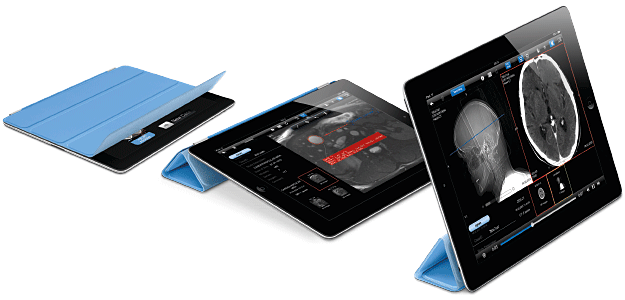
\includegraphics[width=15cm]{images/mobile}~\\
\caption{\label{fig:frog}aycan mobile
}
\end{figure}

Recently, mobile devices, such as PDAs, are being increasingly incorporated to PACS. Typically the flexibility on the visualisation of medical images storage in PACS, offered by a mobile access, is useful in patient care areas and emergency situations. This feature helps healthcare practitioners to have access to medical images at least for a preliminary image analysis in cases where searching for a dedicated terminal to access the images for a detailed and complete analysis is neither practical nor feasible.

\clearpage

The research proposes a distributed system that enables medical image analysis using mobile devices, as well as, the growth in the CAD area combined with the increase in processing power of the mobile devices and in the capacity of wireless networks favours the emergence of new developments integrating those technologies.

The communication between the mobile devices and the image server adopts web service technology \cite{WebService}. To validate the distributed system processing power, speed, and feasibility we develop a tool for medical image analysis with mobile devices dedicated to assist in breast cancer visualisation diagnosis.

The deployed simulation tool allows the medic using a mobile device such as a PDA to determine the evolution of a patient like masses and calcifications location, preventing for instance the need for the doctor to move from analysis machine to the computer. After determine some critical areas, the doctor can visualise the analyse model of the result also using the mobile device. Results show that the use of mobile devices in hospital environments to assist the diagnosis and patient treatment is feasible. Other observation is that the mobile devices can be used to other tasks, like image model rendering, not only image visualisation.